%%%% Paramétrage du TD %%%%
\def\xxactivite{TD 01 \ifprof -- Corrigé \else \fi }
\def\xxauteur{\textsl{Xavier Pessoles}}


\def\xxnumchapitre{Chapitre 1 \vspace{.2cm}}
\def\xxchapitre{\hspace{.12cm} Stabilité des systèmes}

\def\xxcompetences{%
\textsl{%
\textbf{Savoirs et compétences :}\\
\vspace{-.4cm}
\begin{itemize}[label=\ding{112},font=\color{ocre}] 
%\item \textit{Mod3.C2 : } pôles dominants et réduction de l’ordre du modèle : principe, justification
%\item \textit{Res2.C4 : } stabilité des SLCI : définition entrée bornée -- sortie bornée (EB -- SB)	
%\item \textit{Res2.C5 : } stabilité des SLCI : équation caractéristique	
\item \textit{Res2.C6 : } stabilité des SLCI : position des pôles dans le plan complexe
\item \textit{Res2.C7 : } stabilité des SLCI : marges de stabilité (de gain et de phase)
\end{itemize}
}}


\def\xxfigures{
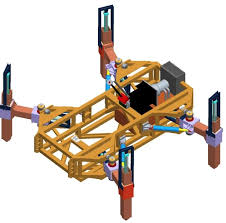
\includegraphics[width=.9\linewidth]{fig_01}
}%figues de la page de garde

\def\xxtitreexo{Drone quadri-rotor}
\def\xxsourceexo{\hspace{.2cm} \footnotesize{\textsl{Pole SII Chateaubriand -- Joliot Curie}}}


\iflivret
\pagestyle{empty}


%%%%%%%% PAGE DE GARDE COURS
\ifcours
\begin{tikzpicture}[remember picture,overlay]
\node at (current page.north west)
{\begin{tikzpicture}[remember picture,overlay]
\node[anchor=north west,inner sep=0pt] at (0,0) {\includegraphics[width=\paperwidth]{\thechapterimage}};
\draw[anchor=west] (-2cm,-8cm) node [line width=2pt,rounded corners=15pt,draw=ocre,fill=white,fill opacity=0.6,inner sep=40pt]{\strut\makebox[22cm]{}};
\draw[anchor=west] (1cm,-8cm) node {\huge\sffamily\bfseries\color{black} %
\begin{minipage}{1cm}
\rotatebox{90}{\LARGE\sffamily\textsc{\color{ocre}\textbf{\xxnumpartie}}}
\end{minipage} \hfill
\begin{minipage}[c]{14cm}
\begin{titrepartie}
\begin{flushright}
\renewcommand{\baselinestretch}{1.1} 
\Large\sffamily\textsc{\textbf{\xxpartie}}
\renewcommand{\baselinestretch}{1} 
\end{flushright}
\end{titrepartie}
\end{minipage} \hfill
\begin{minipage}[c]{3.5cm}
{\large\sffamily\textsc{\textbf{\color{ocre} \discipline}}}
\end{minipage} 
 };
\end{tikzpicture}};
\end{tikzpicture}


\begin{tikzpicture}[overlay]
\node[shape=rectangle, 
      rounded corners = .25 cm,
	  draw= ocre,
	  line width=2pt, 
	  fill = ocre!10,
	  minimum width  = 2.5cm,
	  minimum height = 3cm,] at (18cm,0) {};
\node at (17.7cm,0) {\rotatebox{90}{\textbf{\Large\color{ocre}{\classe}}}};
%{};
\end{tikzpicture}

\vspace{3.5cm}

\begin{tikzpicture}[remember picture,overlay]
\draw[anchor=west] (-2cm,-6cm) node {\huge\sffamily\bfseries\color{black} %
\begin{minipage}{2cm}
\begin{center}
\LARGE\sffamily\textsc{\color{ocre}\textbf{\xxactivite}}
\end{center}
\end{minipage} \hfill
\begin{minipage}[c]{15cm}
\begin{titrechapitre}
\renewcommand{\baselinestretch}{1.1} 
\Large\sffamily\textsc{\textbf{\xxnumchapitre}}

\Large\sffamily\textsc{\textbf{\xxchapitre}}
\vspace{.5cm}

\renewcommand{\baselinestretch}{1} 
\normalsize\normalfont
\xxcompetences
\end{titrechapitre}
\end{minipage}  };
\end{tikzpicture}
\vfill

\begin{flushright}
\begin{minipage}[c]{.3\linewidth}
\begin{center}
\xxfigures
\end{center}
\end{minipage}\hfill
\begin{minipage}[c]{.6\linewidth}
\startcontents
\printcontents{}{1}{}
\end{minipage}
\end{flushright}

\begin{tikzpicture}[remember picture,overlay]
\draw[anchor=west] (4.5cm,-.7cm) node {
\begin{minipage}[c]{.2\linewidth}
\begin{flushright}

\includegraphics[width=2cm]{logoCC}
\end{flushright}
\end{minipage}
\begin{minipage}[c]{.2\linewidth}
\textsl{\xxauteur} \\
\textsl{\classe}
\end{minipage}
 };
\end{tikzpicture}
\newpage
\pagestyle{fancy}

\newpage
\pagestyle{fancy}

\else
\fi


%%%%%%%% PAGE DE GARDE TD
\iftd
%\begin{tikzpicture}[remember picture,overlay]
%\node at (current page.north west)
%{\begin{tikzpicture}[remember picture,overlay]
%\draw[anchor=west] (-2cm,-3.25cm) node [line width=2pt,rounded corners=15pt,draw=ocre,fill=white,fill opacity=0.6,inner sep=40pt]{\strut\makebox[22cm]{}};
%\draw[anchor=west] (1cm,-3.25cm) node {\huge\sffamily\bfseries\color{black} %
%\begin{minipage}{1cm}
%\rotatebox{90}{\LARGE\sffamily\textsc{\color{ocre}\textbf{\xxnumpartie}}}
%\end{minipage} \hfill
%\begin{minipage}[c]{13.5cm}
%\begin{titrepartie}
%\begin{flushright}
%\renewcommand{\baselinestretch}{1.1} 
%\Large\sffamily\textsc{\textbf{\xxpartie}}
%\renewcommand{\baselinestretch}{1} 
%\end{flushright}
%\end{titrepartie}
%\end{minipage} \hfill
%\begin{minipage}[c]{3.5cm}
%{\large\sffamily\textsc{\textbf{\color{ocre} \discipline}}}
%\end{minipage} 
% };
%\end{tikzpicture}};
%\end{tikzpicture}

%%%%%%%%%% PAGE DE GARDE TD %%%%%%%%%%%%%%%
%\begin{tikzpicture}[overlay]
%\node[shape=rectangle, 
%      rounded corners = .25 cm,
%	  draw= ocre,
%	  line width=2pt, 
%	  fill = ocre!10,
%	  minimum width  = 2.5cm,
%	  minimum height = 2.5cm,] at (18.5cm,0) {};
%\node at (17.7cm,0) {\rotatebox{90}{\textbf{\Large\color{ocre}{\classe}}}};
%%{};
%\end{tikzpicture}

% PARTIE ET CHAPITRE
%\begin{tikzpicture}[remember picture,overlay]
%\draw[anchor=west] (-1cm,-2.1cm) node {\large\sffamily\bfseries\color{black} %
%\begin{minipage}[c]{15cm}
%\begin{flushleft}
%\xxnumchapitre \\
%\xxchapitre
%\end{flushleft}
%\end{minipage}  };
%\end{tikzpicture}

% Bandeau titre exo
\begin{tikzpicture}[remember picture,overlay]
\draw[anchor=west] (-2cm,-4cm) node {\huge\sffamily\bfseries\color{black} %
\begin{minipage}{5cm}
\begin{center}
\LARGE\sffamily\color{ocre}\textbf{\textsc{\xxactivite}}

\begin{center}
\xxfigures
\end{center}

\end{center}
\end{minipage} \hfill
\begin{minipage}[c]{12cm}
\begin{titrechapitre}
\renewcommand{\baselinestretch}{1.1} 
\large\sffamily\textbf{\textsc{\xxtitreexo}}

\small\sffamily{\textbf{\textit{\color{black!70}\xxsourceexo}}}
\vspace{.5cm}

\renewcommand{\baselinestretch}{1} 
\normalsize\normalfont
\xxcompetences
\end{titrechapitre}
\end{minipage}  };
\end{tikzpicture}

\else
\fi


%%%%%%%% PAGE DE GARDE FICHE
\iffiche
\begin{tikzpicture}[remember picture,overlay]
\node at (current page.north west)
{\begin{tikzpicture}[remember picture,overlay]
\draw[anchor=west] (-2cm,-3.25cm) node [line width=2pt,rounded corners=15pt,draw=ocre,fill=white,fill opacity=0.6,inner sep=40pt]{\strut\makebox[22cm]{}};
\draw[anchor=west] (1cm,-3.25cm) node {\huge\sffamily\bfseries\color{black} %
\begin{minipage}{1cm}
\rotatebox{90}{\LARGE\sffamily\textsc{\color{ocre}\textbf{\xxnumpartie}}}
\end{minipage} \hfill
\begin{minipage}[c]{14cm}
\begin{titrepartie}
\begin{flushright}
\renewcommand{\baselinestretch}{1.1} 
\large\sffamily\textsc{\textbf{\xxpartie} \\} 

\vspace{.2cm}

\normalsize\sffamily\textsc{\textbf{\xxnumchapitre -- \xxchapitre}}
\renewcommand{\baselinestretch}{1} 
\end{flushright}
\end{titrepartie}
\end{minipage} \hfill
\begin{minipage}[c]{3.5cm}
{\large\sffamily\textsc{\textbf{\color{ocre} \discipline}}}
\end{minipage} 
 };
\end{tikzpicture}};
\end{tikzpicture}


\begin{tikzpicture}[overlay]
\node[shape=rectangle, 
      rounded corners = .25 cm,
	  draw= ocre,
	  line width=2pt, 
	  fill = ocre!10,
	  minimum width  = 2.5cm,
	  minimum height = 2.5cm,] at (18.5cm,0.5cm) {};
%	  minimum height = 2.5cm,] at (18.5cm,0cm) {};
\node at (17.7cm,0.5) {\rotatebox{90}{\textsf{\textbf{\large\color{ocre}{\classe}}}}};
%{};
\end{tikzpicture}



\else
\fi



\else
\pagestyle{empty}


%%%%%%%% PAGE DE GARDE COURS
\ifcours
\begin{tikzpicture}[remember picture,overlay]
\node at (current page.north west)
{\begin{tikzpicture}[remember picture,overlay]
\node[anchor=north west,inner sep=0pt] at (0,0) {\includegraphics[width=\paperwidth]{\thechapterimage}};
\draw[anchor=west] (-2cm,-8cm) node [line width=2pt,rounded corners=15pt,draw=ocre,fill=white,fill opacity=0.6,inner sep=40pt]{\strut\makebox[22cm]{}};
\draw[anchor=west] (1cm,-8cm) node {\huge\sffamily\bfseries\color{black} %
\begin{minipage}{1cm}
\rotatebox{90}{\LARGE\sffamily\textsc{\color{ocre}\textbf{\xxnumpartie}}}
\end{minipage} \hfill
\begin{minipage}[c]{14cm}
\begin{titrepartie}
\begin{flushright}
\renewcommand{\baselinestretch}{1.1} 
\Large\sffamily\textsc{\textbf{\xxpartie}}
\renewcommand{\baselinestretch}{1} 
\end{flushright}
\end{titrepartie}
\end{minipage} \hfill
\begin{minipage}[c]{3.5cm}
{\large\sffamily\textsc{\textbf{\color{ocre} \discipline}}}
\end{minipage} 
 };
\end{tikzpicture}};
\end{tikzpicture}


\begin{tikzpicture}[overlay]
\node[shape=rectangle, 
      rounded corners = .25 cm,
	  draw= ocre,
	  line width=2pt, 
	  fill = ocre!10,
	  minimum width  = 2.5cm,
	  minimum height = 3cm,] at (18cm,0) {};
\node at (17.7cm,0) {\rotatebox{90}{\textbf{\Large\color{ocre}{\classe}}}};
%{};
\end{tikzpicture}

\vspace{3.5cm}

\begin{tikzpicture}[remember picture,overlay]
\draw[anchor=west] (-2cm,-6cm) node {\huge\sffamily\bfseries\color{black} %
\begin{minipage}{2cm}
\begin{center}
\LARGE\sffamily\textsc{\color{ocre}\textbf{\xxactivite}}
\end{center}
\end{minipage} \hfill
\begin{minipage}[c]{15cm}
\begin{titrechapitre}
\renewcommand{\baselinestretch}{1.1} 
\Large\sffamily\textsc{\textbf{\xxnumchapitre}}

\Large\sffamily\textsc{\textbf{\xxchapitre}}
\vspace{.5cm}

\renewcommand{\baselinestretch}{1} 
\normalsize\normalfont
\xxcompetences
\end{titrechapitre}
\end{minipage}  };
\end{tikzpicture}
\vfill

\begin{flushright}
\begin{minipage}[c]{.3\linewidth}
\begin{center}
\xxfigures
\end{center}
\end{minipage}\hfill
\begin{minipage}[c]{.6\linewidth}
\startcontents
\printcontents{}{1}{}
\end{minipage}
\end{flushright}

\begin{tikzpicture}[remember picture,overlay]
\draw[anchor=west] (4.5cm,-.7cm) node {
\begin{minipage}[c]{.2\linewidth}
\begin{flushright}

\includegraphics[width=2cm]{logoCC}
\end{flushright}
\end{minipage}
\begin{minipage}[c]{.2\linewidth}
\textsl{\xxauteur} \\
\textsl{\classe}
\end{minipage}
 };
\end{tikzpicture}
\newpage
\pagestyle{fancy}

\newpage
\pagestyle{fancy}

\else
\fi


%%%%%%%% PAGE DE GARDE TD
\iftd
%\begin{tikzpicture}[remember picture,overlay]
%\node at (current page.north west)
%{\begin{tikzpicture}[remember picture,overlay]
%\draw[anchor=west] (-2cm,-3.25cm) node [line width=2pt,rounded corners=15pt,draw=ocre,fill=white,fill opacity=0.6,inner sep=40pt]{\strut\makebox[22cm]{}};
%\draw[anchor=west] (1cm,-3.25cm) node {\huge\sffamily\bfseries\color{black} %
%\begin{minipage}{1cm}
%\rotatebox{90}{\LARGE\sffamily\textsc{\color{ocre}\textbf{\xxnumpartie}}}
%\end{minipage} \hfill
%\begin{minipage}[c]{13.5cm}
%\begin{titrepartie}
%\begin{flushright}
%\renewcommand{\baselinestretch}{1.1} 
%\Large\sffamily\textsc{\textbf{\xxpartie}}
%\renewcommand{\baselinestretch}{1} 
%\end{flushright}
%\end{titrepartie}
%\end{minipage} \hfill
%\begin{minipage}[c]{3.5cm}
%{\large\sffamily\textsc{\textbf{\color{ocre} \discipline}}}
%\end{minipage} 
% };
%\end{tikzpicture}};
%\end{tikzpicture}

%%%%%%%%%% PAGE DE GARDE TD %%%%%%%%%%%%%%%
%\begin{tikzpicture}[overlay]
%\node[shape=rectangle, 
%      rounded corners = .25 cm,
%	  draw= ocre,
%	  line width=2pt, 
%	  fill = ocre!10,
%	  minimum width  = 2.5cm,
%	  minimum height = 2.5cm,] at (18.5cm,0) {};
%\node at (17.7cm,0) {\rotatebox{90}{\textbf{\Large\color{ocre}{\classe}}}};
%%{};
%\end{tikzpicture}

% PARTIE ET CHAPITRE
%\begin{tikzpicture}[remember picture,overlay]
%\draw[anchor=west] (-1cm,-2.1cm) node {\large\sffamily\bfseries\color{black} %
%\begin{minipage}[c]{15cm}
%\begin{flushleft}
%\xxnumchapitre \\
%\xxchapitre
%\end{flushleft}
%\end{minipage}  };
%\end{tikzpicture}

% Bandeau titre exo
\begin{tikzpicture}[remember picture,overlay]
\draw[anchor=west] (-2cm,-4cm) node {\huge\sffamily\bfseries\color{black} %
\begin{minipage}{5cm}
\begin{center}
\LARGE\sffamily\color{ocre}\textbf{\textsc{\xxactivite}}

\begin{center}
\xxfigures
\end{center}

\end{center}
\end{minipage} \hfill
\begin{minipage}[c]{12cm}
\begin{titrechapitre}
\renewcommand{\baselinestretch}{1.1} 
\large\sffamily\textbf{\textsc{\xxtitreexo}}

\small\sffamily{\textbf{\textit{\color{black!70}\xxsourceexo}}}
\vspace{.5cm}

\renewcommand{\baselinestretch}{1} 
\normalsize\normalfont
\xxcompetences
\end{titrechapitre}
\end{minipage}  };
\end{tikzpicture}

\else
\fi


%%%%%%%% PAGE DE GARDE FICHE
\iffiche
\begin{tikzpicture}[remember picture,overlay]
\node at (current page.north west)
{\begin{tikzpicture}[remember picture,overlay]
\draw[anchor=west] (-2cm,-3.25cm) node [line width=2pt,rounded corners=15pt,draw=ocre,fill=white,fill opacity=0.6,inner sep=40pt]{\strut\makebox[22cm]{}};
\draw[anchor=west] (1cm,-3.25cm) node {\huge\sffamily\bfseries\color{black} %
\begin{minipage}{1cm}
\rotatebox{90}{\LARGE\sffamily\textsc{\color{ocre}\textbf{\xxnumpartie}}}
\end{minipage} \hfill
\begin{minipage}[c]{14cm}
\begin{titrepartie}
\begin{flushright}
\renewcommand{\baselinestretch}{1.1} 
\large\sffamily\textsc{\textbf{\xxpartie} \\} 

\vspace{.2cm}

\normalsize\sffamily\textsc{\textbf{\xxnumchapitre -- \xxchapitre}}
\renewcommand{\baselinestretch}{1} 
\end{flushright}
\end{titrepartie}
\end{minipage} \hfill
\begin{minipage}[c]{3.5cm}
{\large\sffamily\textsc{\textbf{\color{ocre} \discipline}}}
\end{minipage} 
 };
\end{tikzpicture}};
\end{tikzpicture}


\begin{tikzpicture}[overlay]
\node[shape=rectangle, 
      rounded corners = .25 cm,
	  draw= ocre,
	  line width=2pt, 
	  fill = ocre!10,
	  minimum width  = 2.5cm,
	  minimum height = 2.5cm,] at (18.5cm,0.5cm) {};
%	  minimum height = 2.5cm,] at (18.5cm,0cm) {};
\node at (17.7cm,0.5) {\rotatebox{90}{\textsf{\textbf{\large\color{ocre}{\classe}}}}};
%{};
\end{tikzpicture}



\else
\fi



\fi
\setlength{\columnseprule}{.1pt}

\pagestyle{fancy}
\thispagestyle{plain}


\vspace{4.5cm}

\def\columnseprulecolor{\color{ocre}}
\setlength{\columnseprule}{0.4pt} 

%%%%%%%%%%%%%%%%%%%%%%%



\begin{multicols}{2}
\setcounter{exo}{0}
\section*{Présentation}
Cet hélicoptère quadri-rotor à pas fixe est une configuration très répandue dans le monde des microdrones.
Alors que les hélicoptères classiques utilisent un système mécanique complexe de pas cyclique et
collectif, le quadri-rotor ne dispose d'aucun organe mécanique spécifique et assure son contrôle en agissant
uniquement sur la vitesse de rotation de ses rotors. Cette simplicité permet de disposer d'un engin de faible
coût, robuste et facile à miniaturiser.
Le contrôle vertical de l'appareil (translation suivant la direction $\vect{z}$) est obtenu en faisant varier
simultanément la vitesse de rotation des quatre moteurs. Le contrôle en roulis (rotation autour de l’axe $(O,\vect{x})$ ) et en tangage (rotation autour de l’axe $(O,\vect{y})$ ) est obtenu en faisant varier de manière différentielle
les vitesses de rotation des moteurs d'un même axe ($\dfrac{\omega_2}{\omega_4}$  pour le roulis et $\dfrac{\omega_1}{\omega_3}$ pour le tangage).
Un extrait du cahier des charges en phase de décollage est donné ci-dessous.


\begin{center}
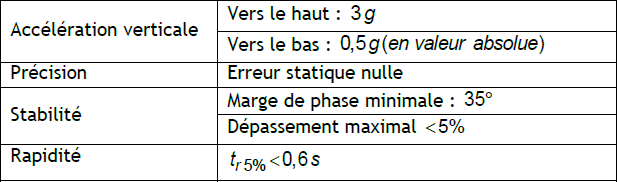
\includegraphics[width=\linewidth]{fig_02}
\end{center}

\begin{obj}
\begin{itemize}
\item Étudier le comportement du quadri-rotor lors du décollage.
\item Vérifier les performances imposées par le cahier des charges.
\end{itemize}
\end{obj}

\section*{Linéarisation du modèle de moteur}
Les moteurs choisis sont des moteurs synchrones sans balais à 14 pôles de type Hacker A20-54 entraînant
directement l'hélice, sans réduction.

\begin{center}
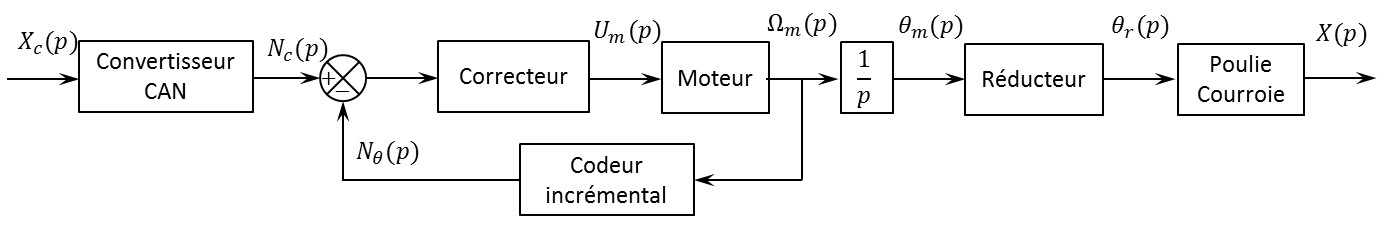
\includegraphics[width=.4\linewidth]{fig_03}
\end{center}

Sous certaines hypothèses simplificatrices, l'équation globale modélisant le moteur et sa commande peut se
mettre sous la forme suivante :
$$
\dfrac{\text{d}\omega(t)}{\text{d}t}=-\dfrac{1}{\tau}\omega(t) -k_q\omega(t)^2 + \dfrac{k_v}{\tau}u.
$$

$u$ représente la tension de commande du moteur, $\omega(t)$ son taux de rotation, $\tau$ et $k_v$ des constantes caractéristiques de l'ensemble moteur-hélice. Le terme $k_q\omega^2$ provient du couple de frottement aérodynamique de l'air sur l'hélice tournant à grande vitesse.

L'équation du modèle du moteur fait apparaître un terme non linéaire en $\omega^2$, qui nécessite de linéariser
donc l'équation autour du point de fonctionnement $\omega_0$, fréquence de rotation du moteur qui permet de
maintenir le mini-drone en équilibre en vol stationnaire.

On pose $\omega=\omega_0+\delta \omega$ et $u=u_0+\delta u$ où $\delta\omega$ et $\delta u$ représentent des petites variations de $\omega$ et $u$ autour du point de fonctionnement.

\subparagraph{}\textit{Déterminer l’équation stationnaire liant $\omega_0$ et $u_0$.}

\subparagraph{}\textit{Montrer que l'équation différentielle liant $\delta \omega$ et $\delta u$ est de la forme $\dfrac{\text{d}\delta \omega(t) }{\text{d}t}=-A\delta \omega(t) + B \delta u$. Exprimer $A$ et $B$ en fonction des paramètres $\tau$, $k_v$, $k_q$ et $\omega_0$.}

On note $\Delta \Omega (p)$ la transformée de Laplace de $\delta \omega$ et $\Delta U(p)$ celle de $\delta u$.


\subparagraph{}\textit{Calculer la fonction de transfert $\dfrac{\Delta{\Omega(s)}}{\Delta U(s)}$ du moteur. Donner l'expression de ses paramètres caractéristiques $K_m$ et $T_m$ en fonction des paramètres $\tau$, $k_v$, $k_q$ et $\omega_0$.}

\section*{Recherche du point de fonctionnement $\omega_0$}
Dans le mouvement de déplacement vertical de direction $\vect{z}$ , les quatre moteurs tournent à la même vitesse et fournissent la même poussée $F=F_1=F_2=F_3=F_4$.
La masse totale du drone est $m=\SI{240}{g}$. On prendra $g=\SI{9,81}{m.s^{-2}}$.

\subparagraph{}\textit{Calculer numériquement la poussée $F_0$ que doit exercer chacun des quatre moteurs pour maintenir l’appareil en vol stationnaire à l’altitude $z_0$ .}

La poussée $F$ varie avec $\omega^2$ . Des mesures réalisées sur un seul groupe moteur-hélice ont permis de tracer la courbe liant $F$ à la fréquence de rotation $\omega$ en rad/s.

\begin{center}
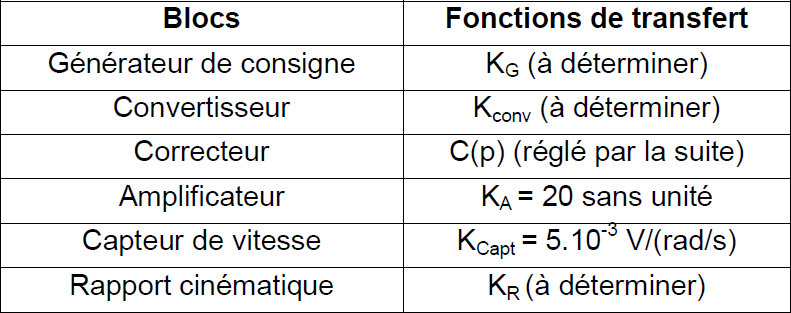
\includegraphics[width=\linewidth]{fig_04}
\end{center}

\subparagraph{}\textit{Déterminer la fréquence de rotation $\omega_0$ des
moteurs en vol stationnaire.}




Des essais ont également permis de tracer la
courbe liant la tension de commande $u$ et la
fréquence de rotation $\omega$ en rad/s en régime
permanent lorsque $\dfrac{\text{d}\omega(t)}{\text{d}(t)}=0$. La courbe de tendance associée aux résultats de
ces essais est de la forme $y=ax^2+bx$. On donne la constante de temps du moteur :
$\tau=\SI{125}{ms}$.

\begin{center}
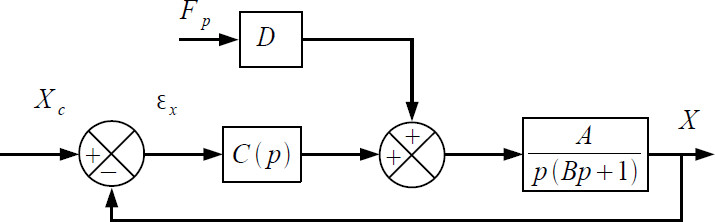
\includegraphics[width=\linewidth]{fig_05}
\end{center}

\subparagraph{}\textit{Déterminer l'expression des coefficients $k_v$ et $k_q$ en fonction de $a$, $b$ et $\tau$. Préciser leur unité.}

On peut ainsi déduire le modèle $\dfrac{\Delta \Omega(p)}{\Delta U(p)}$ du moteur linéarisé autour de son point de fonctionnement. Pour la suite, on retiendra le modèle suivant : $\dfrac{\Delta \Omega(p)}{\Delta U(p)}=\dfrac{37,5}{1+\dfrac{p}{77}}$.

\section*{Vérification des performances}

L'asservissement vertical du drone peut être représente après linéarisation des différentes fonctions de
transfert autour du point de fonctionnement $\omega_0$, par le schéma-bloc suivant :

\begin{center}
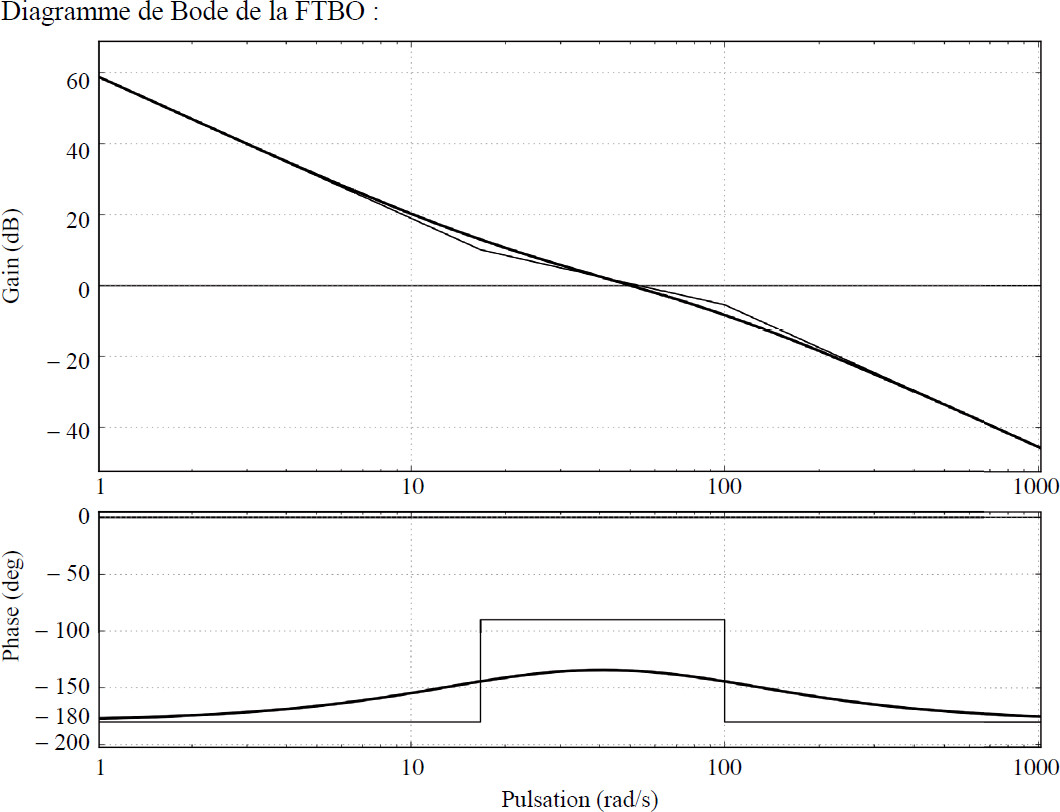
\includegraphics[width=\linewidth]{fig_06}
\end{center}



Le gain du capteur barométrique est de $\SI{0,05}{V.m^{-1}}$. On pose $z=z_0+\Delta z(p)$, la transformée de Laplace de $\delta Z$, $F=F_0 + \delta F$ représente la poussée d'un seul moteur et on utilise l'équation linéarisée avec conditions initiales nulles.

Le théorème de la résultante dynamique, en projection sur l’axe vertical, permet d’écrire :
$$ m\ddot{z} =4F-mg. $$


\subparagraph{}\textit{Déterminer la fonction de transfert $\dfrac{\Delta Z(p)}{\Delta F(p)}$ à partir de l'équation du principe fondamental de la dynamique. En déduire l'expression de la fonction de transfert en boucle ouverte. }


Dans la suite, le gain de la fonction de transfert en boucle ouverte sera noté $K_{BO}=2,5 K$.
La courbe de phase du diagramme de Bode de la fonction de transfert en boucle ouverte est représentée ci-dessous, en gras avec un correcteur proportionnel ($T=0$) et en trait fin avec le correcteur retenu ($K=1$ et $T=0,2s$).


\begin{center}
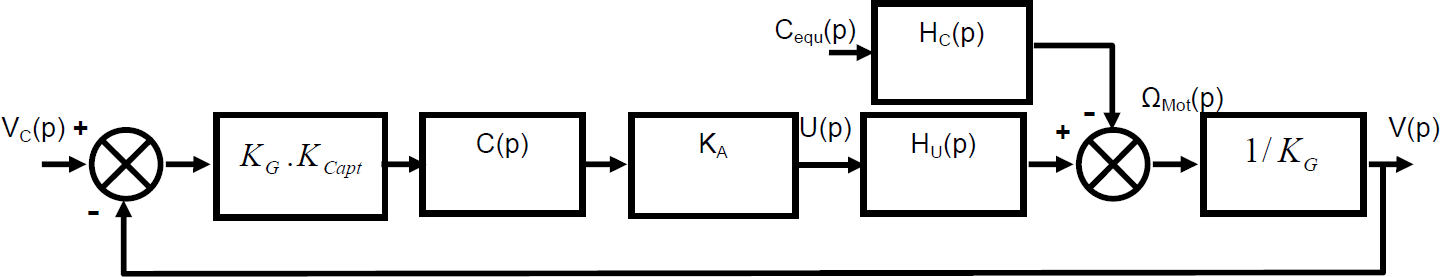
\includegraphics[width=\linewidth]{fig_07}
\end{center}


\subparagraph{}\textit{Tracer le diagramme asymptotique de la courbe de gain avec le correcteur $T=\SI{0,2}{s}$ et $K=1$.
Préciser les pentes et les pulsations de brisure. Le diagramme sera tracé entre 1 et \SI{1000}{rad.s^{-1}}, le gain sera compris entre \SI{-120}{dB} et \SI{+10}{dB}.}

\subparagraph{}\textit{Justifier que pour $K=1$, on a $\omega=\SI{1,5}{rad.s^{-1}}$. En déduire graphiquement la marge de phase pour
$K=1$. Commenter.}

\subparagraph{}\textit{Procéder au réglage du gain $K$ du correcteur afin d’assurer le respect du critère de stabilité du cahier des charges.}

\subparagraph{}\textit{Le critère de précision du cahier des charges est-il vérifié ? Justifier.}

La figure suivante représente la position des pôles de la fonction de transfert en boucle fermée dans le plan
complexe, pour la valeur du gain $K$ précédemment déterminée.


\begin{center}
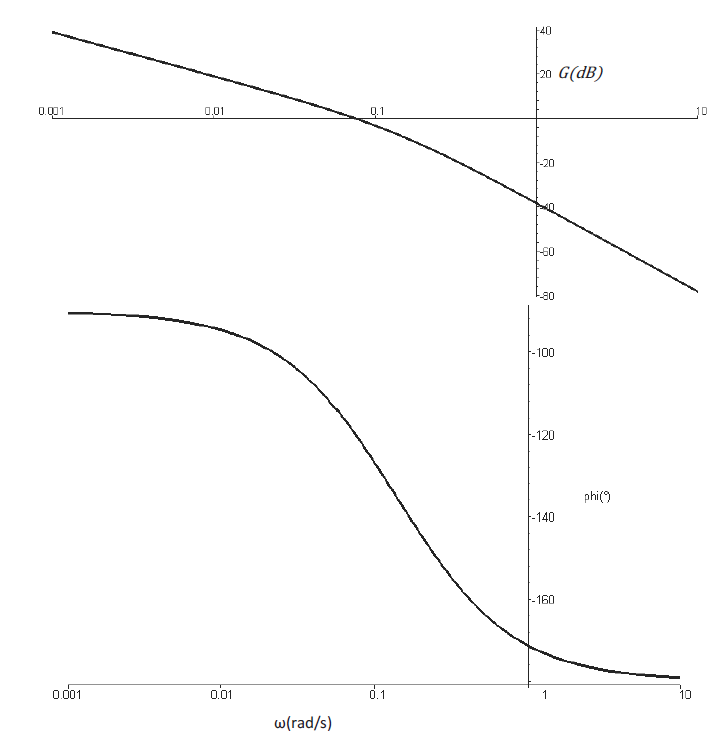
\includegraphics[width=\linewidth]{fig_08}
\end{center}


\subparagraph{}\textit{Repérer le(s) pôle(s) dominant(s) et donner sa (leur) valeur(s) numérique(s).}

\subparagraph{}\textit{À l’aide des droites d’iso-amortissement, indiquer la valeur du coefficient d’amortissement $\xi$ de la
fonction de transfert du deuxième ordre pouvant modéliser l’asservissement vertical du drone lorsque
l’on néglige les autres pôles par rapport à ces pôles dominants.}

\subparagraph{}\textit{En déduire la présence ou l’absence d’oscillations verticales du drone lors d’un décollage supposé
modélisé par un échelon d’amplitude 1 mètre. Le critère de stabilité est-il intégralement vérifié ?}

\subparagraph{}\textit{Donner l’expression littérale des pôles d’un système du deuxième ordre de pulsation propre $\omega_n$ et de coefficient d’amortissement $\xi<1$. En déduire une estimation de la pulsation propre $\omega_n$ de la
fonction de transfert approchée de l’asservissement vertical du drone.}

\subparagraph{}\textit{Vérifier si le critère de rapidité du cahier des charges est vérifié.}

\begin{center}
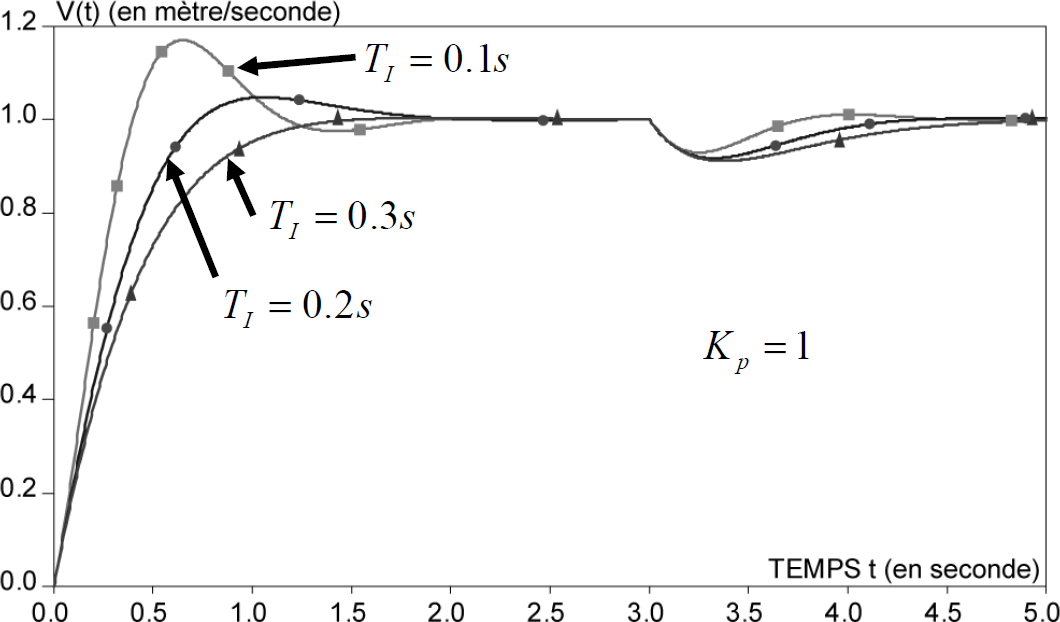
\includegraphics[width=\linewidth]{fig_09}
\end{center}



%\begin{multicols}
%\newpage


Pour éventuellement vous aider....
\begin{enumerate}
\item $-\dfrac{1}{\tau}\omega_0 - k_q \omega_0^2 + \dfrac{k_v}{\tau}u_0=0$;
\item $A=\dfrac{1}{\tau}+2k_q\omega_0$ et $B=\dfrac{k_v}{\tau}$.
\item $K_m=\dfrac{k_v}{1+2\tau k_q \omega_0}$ et $T_m=\dfrac{\tau}{1+2\tau k_q \omega_0}$.
\item $F_0=\dfrac{mg}{4}=\SI{0,6}{N}$
\item $\omega_0=\SI{340}{rad.s^{-1}}$
\item $k_v=\dfrac{1}{b}$ (rad/s/V) et $k_b=\dfrac{a}{b\tau}$
\item $\dfrac{\Delta Z(p)}{\Delta F(p)}=\dfrac{4}{mp^2}$. $H_{BO}(p)=\dfrac{2,5 K}{p^2}\dfrac{1+Tp}{\left( 1+\dfrac{p}{77}\right)\left(1+\dfrac{p}{30} \right)}$ 
\item  $\quad$
\item $\quad$
\item $K=17,9$.
\item La FTBO est de classe 2, l'erreur de position est donc nulle.
\item $p_2=-15$, $p_3 = -5+8j$, $p_4=-5+8j$.
\item $\xi=0,6$
\item $\quad$
\item $p=-\xi\omega_n \pm j\omega_n \sqrt{1-\xi^2}$. $\omega_n\simeq \SI{8,33}{rad.s^{-1}}$
\item $t_{5\%}\simeq \SI{0,61}{ s}$. 
\end{enumerate}
\end{multicols}

%\end{document}
%
%\subparagraph{}\textit{}
%
%
%\begin{center}
%\includegraphics[width=\linewidth]{}
%\end{center}
%
%\begin{center}
%\includegraphics[width=\linewidth]{}
%\textit{}
%\end{center}
%
